\def\version{1}
\problemname{Labyrintkonstruktion}
Låt oss definiera en \textit{labyrint} på följande sätt:
\begin{enumerate}
  \item Labyrinten består av $K$ rum, där vissa par av rum är sammanbundna av korridorer.
  \item Det går att ta sig mellan alla par av rum om man går genom en sekvens av korridorer.
  \item Inget rum har en korridor till sig själv.
  \item Det kan finnas flera korridorer som kopplar samman samma par av rum.
  \item Varje korridor har en av tre färger: röd, grön eller blå.
  \item Varje rum har exakt tre korridorer, en av varje färg.
  \item Det finns ett rum som är labyrintens ingång, och ett rum som är labyrintens utgång (dessa är olika rum).
\end{enumerate}

Systrarna Rosa och Lila spelar ett spel som går ut på att Rosa först konstruerar en labyrint, varpå Lila försöker klara av den genom att gå från ingången till utgången.
De har spelat några gånger nu, och Lila lyckas alltid vinna.
Detta gör Rosa ganska frustrerad.
Hon vill att hennes syster ska fastna i labyrinten för alltid.

Rosa har dock märkt att Lila alltid använder samma förutsägbara strategi.
Närmare bestämt har hon en sträng $S$ med längden $L$, bestående av bokstäverna \texttt{R}, \texttt{G} och \texttt{B} (röd, grön och blå).
I drag nummer $i$ tittar Lila på det $i$:te tecknet, och följer korridoren med den färg som bokstaven representerar (om bokstaven är \texttt{R} kommer Lila alltså gå genom den röda korridoren i det rum hon befinner sig i just nu).
Efter $L$ drag börjar hon om genom att titta på det första tecknet igen.
Om strängen är \texttt{RGB} kommer hon med andra ord först gå genom den röda korridoren i ingången, sedan den gröna korridoren i rummet hon kom till, sedan den blå korridoren, den röda (nu har hon börjat läsa strängen från början igen), gröna, blå, röda, och så vidare.
Notera att varje rum har exakt en korridor av varje färg, så det är unikt bestämt vilket rum hon går till i varje steg.

\begin{figure}[h!]
  \centering
  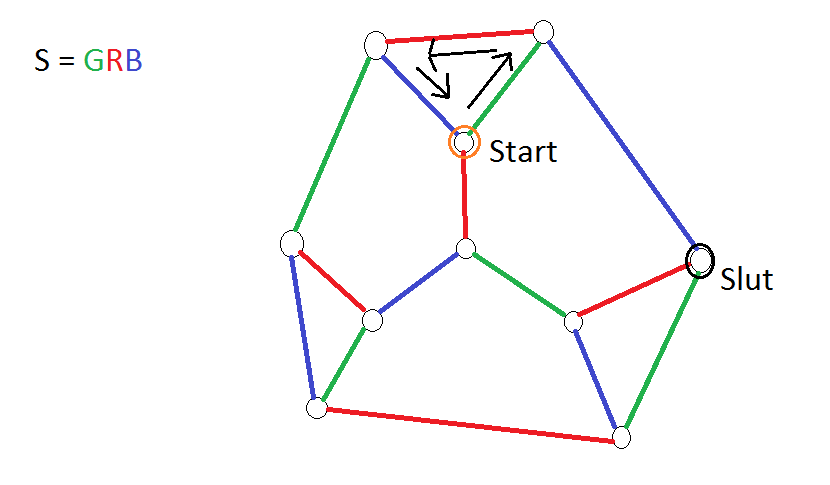
\includegraphics[width=0.6\textwidth]{labyrintgraf2.png}
  \caption{En exempellabyrint.}
\end{figure}

Din uppgift är att, givet $S$, konstruera en labyrint som Lila aldrig kan klara av.

\section*{Indata}
Indatan innehåller strängen $S$ av längd minst $1$ och högst $1\,000\,000$.

I detta problem kan du dessutom ladda ner all indata här: \url{http://progolymp.se/uploads/labyrint.zip}.

\section*{Utdata}
Börja med att skriva ut tre heltal $K$, $i$, $u$.
$K$ ska vara antalet rum i labyrinten du konstruerar.
$i$ och $u$ ska vara de noll-indexerade nummer (d.v.s mellan $0$ och $K - 1$) på rummen som är ingången och utgången i labyrinten.

Skriv sedan ut $K$ rader, ett för varje rum.
Den $j$:te raden ska innehålla tre heltal $r$, $g$ och $b$ -- de rum som den röda, gröna respektive blå korridoren i det $j$:te rummet leder till.

Din labyrint måste uppfylla villkoren i problemlydelsen.

\section*{Poängsättning}
Totalt har problemet 10 testfall.

Låt $minK$ vara antalet rum i den minsta labyrinten någon deltagare lyckas konstruera på ett visst testfall, och $K$ antalet rum i din labyrint.
Låt
$$r_1 = \frac{K}{minK}$$
och
$$r_2 = \frac{2|S|}{minK}$$
där $|S|$ är längden på strängen $S$.

Din poäng på det testfallet är då
$$10 \cdot \left(1 - \frac{\log(r_1)}{\log(r_2)}\right)$$,
eller 0 om K överstiger $2|S|$.

Under tävlingen kommer $minK$ sättas till ett värde beräknat utifrån en domarlösning.
